\documentclass{article}
\usepackage{tikz}
\usetikzlibrary{arrows.meta,positioning,calc,shapes.geometric}
\pagestyle{empty}
\begin{document}
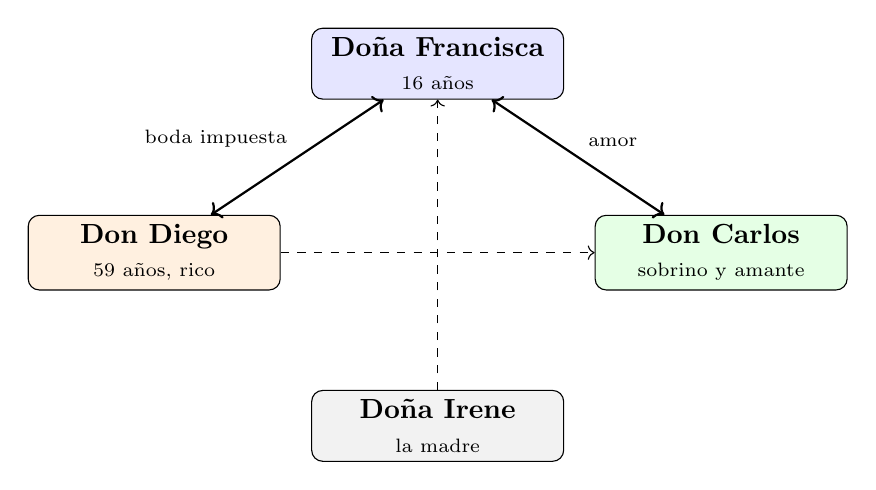
\begin{tikzpicture}
\tikzset{every node/.append style={align=center}}

\node[draw, rounded corners, fill=blue!10, minimum width=3.2cm, align=center] (f) at (0,2.4) {\textbf{Doña Francisca}\\ \scriptsize 16 años};
\node[draw, rounded corners, fill=orange!12, minimum width=3.2cm, align=center] (d) at (-3.6,0) {\textbf{Don Diego}\\ \scriptsize 59 años, rico};
\node[draw, rounded corners, fill=green!10, minimum width=3.2cm, align=center] (c) at (3.6,0) {\textbf{Don Carlos}\\ \scriptsize sobrino y amante};
\node[draw, rounded corners, fill=gray!10, minimum width=3.2cm, align=center] (i) at (0,-2.2) {\textbf{Doña Irene}\\ \scriptsize la madre};
\draw[<->, thick] (f) -- node[above left, font=\scriptsize]{boda impuesta} (d);
\draw[<->, thick] (f) -- node[above right, font=\scriptsize]{amor} (c);
\draw[->, dashed] (i) -- (f);
\draw[->, dashed] (d) -- (c);

\end{tikzpicture}
\end{document}
